\documentclass{beamer}
\usepackage{tikz}
\usepackage{drawstack}
\usepackage{graphicx}

\usetikzlibrary{graphs,quotes,arrows,automata}

\mode<presentation>
\usefonttheme{serif}

\beamertemplatenavigationsymbolsempty
\setbeamertemplate{footline}[frame number]

\definecolor{lightred}{rgb}{0.8,0.8,1}
\definecolor{lightgrey}{rgb}{0.8,0.8,0.8}

\title{Verified double-hashing hash map}
\author{Martin \textsc{Vassor}}

\institute[\'Ecole polytechnique f\'ed\'erale de Lausanne] 
{
  DSLab, EPFL
  \vspace{0.5cm}

  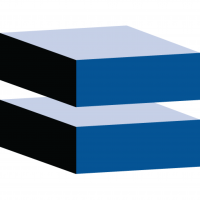
\includegraphics[height=1cm]{DSLab.png}
  \hspace{0.1cm}
  
\includegraphics[height=1cm]{epfl.eps}
}


\newcommand{\keyvalue}[2] {
	\begin{tabular}{| p{0.8cm} | p{1.3cm} |}
			\hline
			\texttt{#1} & \texttt{#2} \\
			\hline
		\end{tabular}
}

\begin{document}

\subject{Verified double-hashed hash table}
\AtBeginSection[] {
  \begin{frame}<beamer>{Outline}
    \tableofcontents[currentsection,currentsubsection]
  \end{frame}
} 

\begin{frame}
\titlepage
\end{frame}

\begin{frame}{Outline}
	\tableofcontents
	
\end{frame}

\section{Introduction}
\begin{frame}
	\frametitle{Naive hash table}
	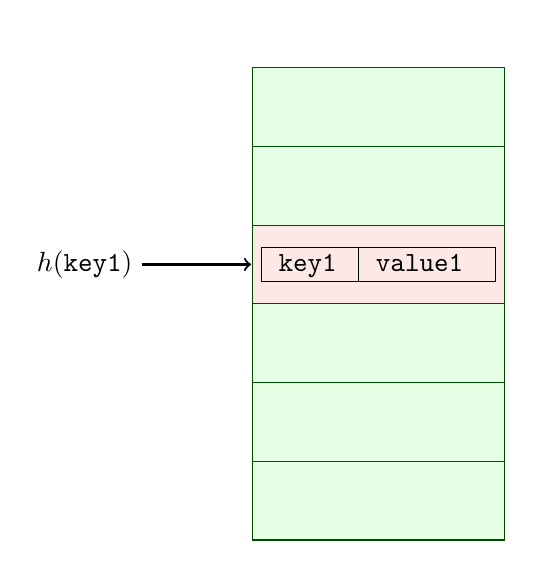
\begin{tikzpicture}
		\draw (0, -3) node[anchor=east] (key1) {$h(\mathtt{key1})$};

		\drawstruct{(3,0)}
		\structcell[freecell]{} \coordinate(firstCell) at (currentcell.east) ;
		\structcell[freecell]{} \coordinate(secondCell) at (currentcell.east);
		\structcell[occupiedcell]{\keyvalue{key1}{value1}} \coordinate(thirdCell) at (currentcell.west);
		\structcell[freecell]{} \coordinate(fourthCell) at (currentcell.east);
		\structcell[freecell]{} \coordinate(fifthCell) at (currentcell.east);
		\structcell[freecell]{} \coordinate(sixthCell) at (currentcell.east);

		\draw[->, thick] (key1) -- (thirdCell);
	\end{tikzpicture}

\end{frame}

\begin{frame}
	\frametitle{Naive hash table}
	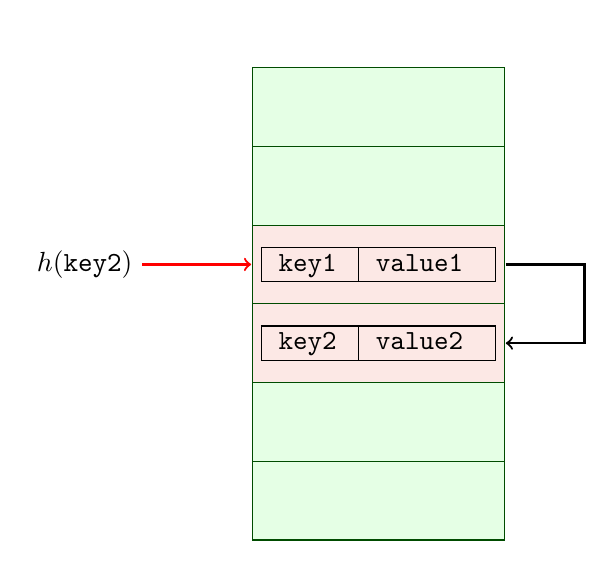
\begin{tikzpicture}
		\draw (0, -3) node[anchor=east] (key2) {$h(\mathtt{key2})$};

		\drawstruct{(3,0)}
		\structcell[freecell]{} \coordinate(firstCell) at (currentcell.east) ;
		\structcell[freecell]{} \coordinate(secondCell) at (currentcell.east);
		\structcell[occupiedcell]{\keyvalue{key1}{value1}} \coordinate(thirdCell) at (currentcell.west); \coordinate(thirdCellOut) at (currentcell.east);
		\structcell[occupiedcell]{\keyvalue{key2}{value2}} \coordinate(fourthCell) at (currentcell.east); \coordinate(fourthCellOut) at (currentcell.east);
		\structcell[freecell]{} \coordinate(fifthCell) at (currentcell.east);
		\structcell[freecell]{} \coordinate(sixthCell) at (currentcell.east);

		\draw[->, red, thick] (key2) -- (thirdCell);
		\draw[->, thick] (thirdCellOut) -- ++(1, 0) |- (fourthCellOut);
	\end{tikzpicture}
\end{frame}

\begin{frame}
	\frametitle{Naive hash table}
	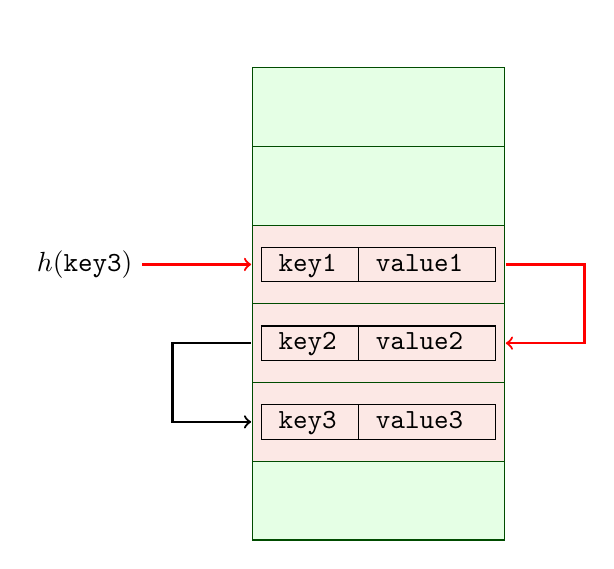
\begin{tikzpicture}
		\draw (0, -3) node[anchor=east] (key3) {$h(\mathtt{key3})$};

		\drawstruct{(3,0)}
		\structcell[freecell]{} \coordinate(firstCell) at (currentcell.east) ;
		\structcell[freecell]{} \coordinate(secondCell) at (currentcell.east);
		\structcell[occupiedcell]{\keyvalue{key1}{value1}} \coordinate(thirdCell) at (currentcell.west); \coordinate(thirdCellOut) at (currentcell.east);
		\structcell[occupiedcell]{\keyvalue{key2}{value2}} \coordinate(fourthCell) at (currentcell.west); \coordinate(fourthCellOut) at (currentcell.east);
		\structcell[occupiedcell]{\keyvalue{key3}{value3}} \coordinate(fifthCell) at (currentcell.west); \coordinate(fifthCellOut) at (currentcell.east);
		\structcell[freecell]{} \coordinate(sixthCell) at (currentcell.east);

		\draw[->, red, thick] (key3) -- (thirdCell);
		\draw[->, red, thick] (thirdCellOut) -- ++(1, 0) |- (fourthCellOut);
		\draw[->, thick] (fourthCell) -- ++(-1, 0) |- (fifthCell);
	\end{tikzpicture}
\end{frame}

\begin{frame}
	\frametitle{Double hashing}
	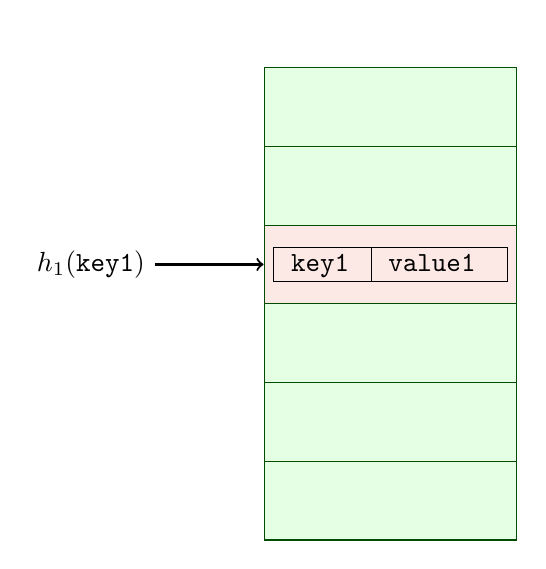
\begin{tikzpicture}
		\draw (0, -3) node[anchor=east] (key1) {$h_1(\mathtt{key1})$};

		\drawstruct{(3,0)}
		\structcell[freecell]{} \coordinate(firstCell) at (currentcell.east) ;
		\structcell[freecell]{} \coordinate(secondCell) at (currentcell.east);
		\structcell[occupiedcell]{\keyvalue{key1}{value1}} \coordinate(thirdCell) at (currentcell.west);
		\structcell[freecell]{} \coordinate(fourthCell) at (currentcell.east);
		\structcell[freecell]{} \coordinate(fifthCell) at (currentcell.east);
		\structcell[freecell]{} \coordinate(sixthCell) at (currentcell.east);

		\draw[->, thick] (key1) -- (thirdCell);
	\end{tikzpicture}

\end{frame}

\begin{frame}
	\frametitle{Double hashing}
	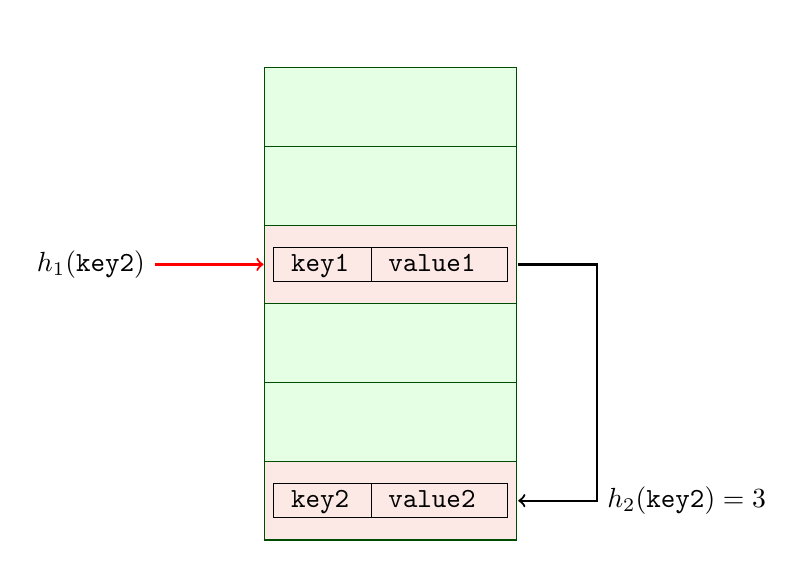
\begin{tikzpicture}
		\draw (0, -3) node[anchor=east] (key2) {$h_1(\mathtt{key2})$};

		\drawstruct{(3,0)}
		\structcell[freecell]{} \coordinate(firstCell) at (currentcell.east) ;
		\structcell[freecell]{} \coordinate(secondCell) at (currentcell.east);
		\structcell[occupiedcell]{\keyvalue{key1}{value1}} \coordinate(thirdCell) at (currentcell.west); \coordinate(thirdCellOut) at (currentcell.east);
		\structcell[freecell]{} \coordinate(fourthCell) at (currentcell.east); \coordinate(fourthCellOut) at (currentcell.east);
		\structcell[freecell]{} \coordinate(fifthCell) at (currentcell.east);
		\structcell[occupiedcell]{\keyvalue{key2}{value2}} \coordinate(sixthCell) at (currentcell.east); \coordinate(sixthCellOut) at (currentcell.east);

		\draw[->, red, thick] (key2) -- (thirdCell);
		\draw[->, thick] (thirdCellOut) -- ++(1, 0) |- (sixthCellOut) node [pos=0.5, anchor=west] {$h_2(\mathtt{key2}) = 3$};
	\end{tikzpicture}
\end{frame}

\begin{frame}
	\frametitle{Double hashing}
	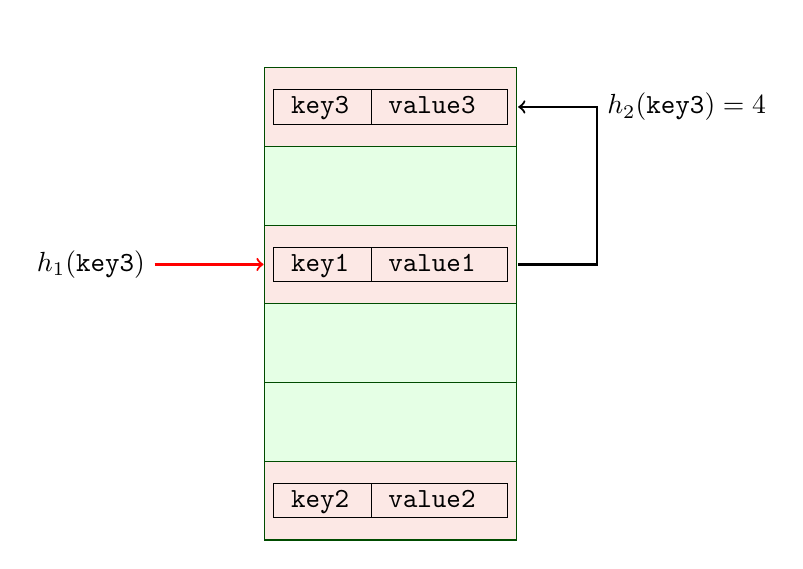
\begin{tikzpicture}
		\draw (0, -3) node[anchor=east] (key3) {$h_1(\mathtt{key3})$};

		\drawstruct{(3,0)}
		\structcell[occupiedcell]{\keyvalue{key3}{value3}} \coordinate(firstCell) at (currentcell.east) ; \coordinate(firstCellOut) at (currentcell.east);
		\structcell[freecell]{} \coordinate(secondCell) at (currentcell.east);
		\structcell[occupiedcell]{\keyvalue{key1}{value1}} \coordinate(thirdCell) at (currentcell.west); \coordinate(thirdCellOut) at (currentcell.east);
		\structcell[freecell]{} \coordinate(fourthCell) at (currentcell.east); \coordinate(fourthCellOut) at (currentcell.east);
		\structcell[freecell]{} \coordinate(fifthCell) at (currentcell.west); \coordinate(fifthCellOut) at (currentcell.east);
		\structcell[occupiedcell]{\keyvalue{key2}{value2}} \coordinate(sixthCell) at (currentcell.east); \coordinate(sixthCellOut) at (currentcell.east);

		\draw[->, red, thick] (key3) -- (thirdCell);
		\draw[->, thick] (thirdCellOut) -- ++(1, 0) |- (firstCellOut) node [pos=0.5, anchor=west] {$h_2(\mathtt{key3})=4$};
	\end{tikzpicture}
\end{frame}

\begin{frame}
	\frametitle{Provided implementation}
	\begin{itemize}
		\item A naive implementation
		\item \texttt{findEmpty}, \texttt{findKey} perform the loops.
	\end{itemize}
\end{frame}

\begin{frame}
	\frametitle{Provided verification}
	Example: successful search of \texttt{key3}
	\begin{center}
		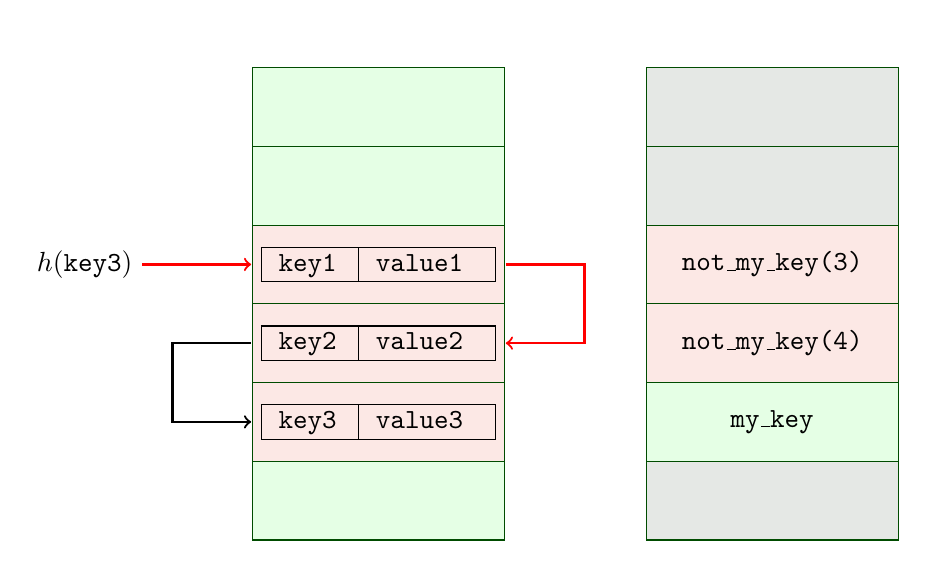
\begin{tikzpicture}
			\draw (0, -3) node[anchor=east] (key3) {$h(\mathtt{key3})$};

			\drawstruct{(8,0)}
			\structcell[padding]{} ;
			\structcell[padding]{} ;
			\structcell[occupiedcell]{\texttt{not\_my\_key(3)}} ;
			\structcell[occupiedcell]{\texttt{not\_my\_key(4)}} ; \coordinate(fourthCellOut) at (currentcell.east);
			\structcell[freecell]{\texttt{my\_key}} ;
			\structcell[padding]{} ;

			\drawstruct{(3,0)}
			\structcell[freecell]{} \coordinate(firstCell) at (currentcell.east) ;
			\structcell[freecell]{} \coordinate(secondCell) at (currentcell.east);
			\structcell[occupiedcell]{\keyvalue{key1}{value1}} \coordinate(thirdCell) at (currentcell.west); \coordinate(thirdCellOut) at (currentcell.east);
			\structcell[occupiedcell]{\keyvalue{key2}{value2}} \coordinate(fourthCell) at (currentcell.west); \coordinate(fourthCellOut) at (currentcell.east);
			\structcell[occupiedcell]{\keyvalue{key3}{value3}} \coordinate(fifthCell) at (currentcell.west); \coordinate(fifthCellOut) at (currentcell.east);
			\structcell[freecell]{} \coordinate(sixthCell) at (currentcell.east);

			\draw[->, red, thick] (key3) -- (thirdCell);
			\draw[->, red, thick] (thirdCellOut) -- ++(1, 0) |- (fourthCellOut);
			\draw[->, thick] (fourthCell) -- ++(-1, 0) |- (fifthCell);
		\end{tikzpicture}
	\end{center}
\end{frame}

\begin{frame}
	\frametitle{Provided verification}
	Example: unsuccessful search of \texttt{key4}
	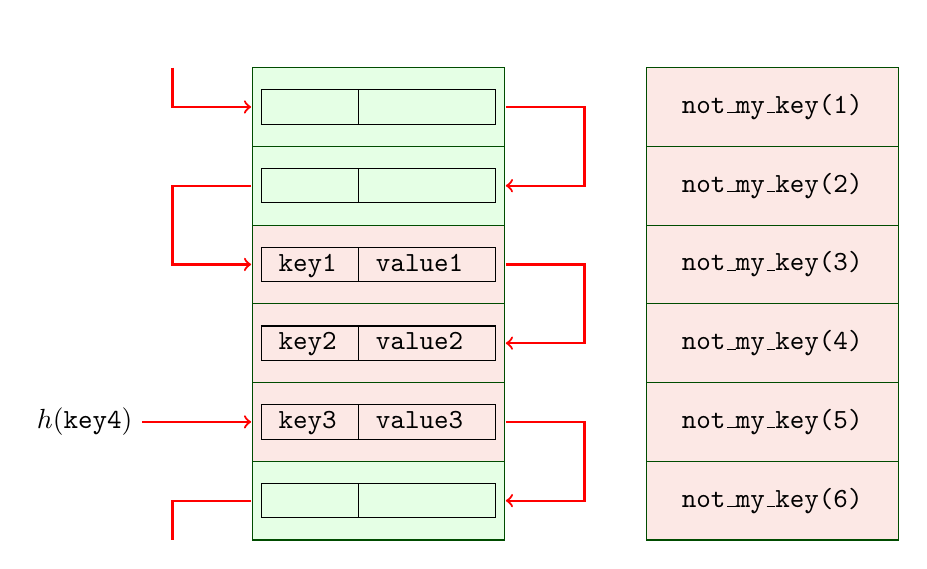
\begin{tikzpicture}
		\draw (0, -5) node[anchor=east] (key4) {$h(\mathtt{key4})$};

		\drawstruct{(8,0)}
		\structcell[occupiedcell]{\texttt{not\_my\_key(1)}} ;
		\structcell[occupiedcell]{\texttt{not\_my\_key(2)}} ;
		\structcell[occupiedcell]{\texttt{not\_my\_key(3)}} ;
		\structcell[occupiedcell]{\texttt{not\_my\_key(4)}} ;
		\structcell[occupiedcell]{\texttt{not\_my\_key(5)}} ;
		\structcell[occupiedcell]{\texttt{not\_my\_key(6)}} ;

		\drawstruct{(3,0)}
		\structcell[freecell]{\keyvalue{}{}} \coordinate(firstCell) at (currentcell.west) ; \coordinate(firstCellOut) at (currentcell.east);
		\structcell[freecell]{\keyvalue{}{}} \coordinate(secondCell) at (currentcell.west); \coordinate (secondCellOut) at (currentcell.east);
		\structcell[occupiedcell]{\keyvalue{key1}{value1}} \coordinate(thirdCell) at (currentcell.west); \coordinate(thirdCellOut) at (currentcell.east);
		\structcell[occupiedcell]{\keyvalue{key2}{value2}} \coordinate(fourthCell) at (currentcell.west); \coordinate(fourthCellOut) at (currentcell.east);
		\structcell[occupiedcell]{\keyvalue{key3}{value3}} \coordinate(fifthCell) at (currentcell.west); \coordinate(fifthCellOut) at (currentcell.east);
		\structcell[freecell]{\keyvalue{}{}} \coordinate(sixthCell) at (currentcell.west); \coordinate (sixthCellOut) at (currentcell.east);

		\draw[->, red, thick] (key4) -- (fifthCell);
		\draw[->, red, thick] (thirdCellOut) -- ++(1, 0) |- (fourthCellOut);
		\draw[->, red, thick] (fifthCellOut) -- ++ (1, 0) |- (sixthCellOut);
		\draw[red, thick] (sixthCell) -| ++(-1, -0.5);
		\draw[->, red, thick] (firstCell)+(-1, 0.5) |- (firstCell);
		\draw[->, red, thick] (firstCellOut) -- ++(1, 0) |- (secondCellOut);
		\draw[->, red, thick] (secondCell) -- ++(-1, 0) |- (thirdCell);
	\end{tikzpicture}
\end{frame}

\begin{frame}
	\frametitle{Provided verification}
	Part before and after ``$\forall i. \mathtt{not\_my\_key(i)} = true$'' provided.\\
	\vspace{1cm}
	For insertion: 
	\begin{itemize}
		\item Same idea
		\item Property: \texttt{findEmpty}
	\end{itemize}
\end{frame}

\section{Implementation}
\subsection{Modifications}
\begin{frame}
	\frametitle{Modifications}

	\begin{itemize}
		\item 64 bits hashes.
	\end{itemize}
	\begin{center}
		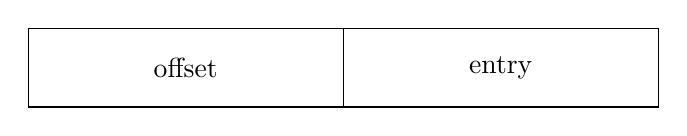
\begin{tikzpicture}
			\draw (0,0) rectangle (4, 1) node[pos=0.5] {offset};
			\draw (4,0) rectangle (8, 1) node[pos=0.5] {entry};
		\end{tikzpicture}
	\end{center}
	
	Except type changes, only \texttt{for} loops modified.

\end{frame}
\subsection{Performance evaluation}
\begin{frame}
	\frametitle{Performance evaluation}
	\begin{itemize}
		\item Build a benchmark tool.
		\item Size, number of accesses, load, read/write ratio, etc\ldots
		\item Converter to C file.
		\item First warms-up, then measures when target load is reached.
	\end{itemize}
	
	\vspace{0.5cm}
	\begin{center}
		\texttt{test\_load.sh length read\_ratio load1 [load2\ldots]}
	\end{center}

\end{frame}

\begin{frame}
	\frametitle{Evaluation cases}
	\begin{itemize}
		\item Worst case: searching a non existing element.
	\end{itemize}

	\begin{enumerate}
		\item Allow searching non existing element.
		\item Search only existing element.
	\end{enumerate}
\end{frame}

\subsection{Performance results}
\begin{frame}
	\frametitle{Result}
	\begin{center}
		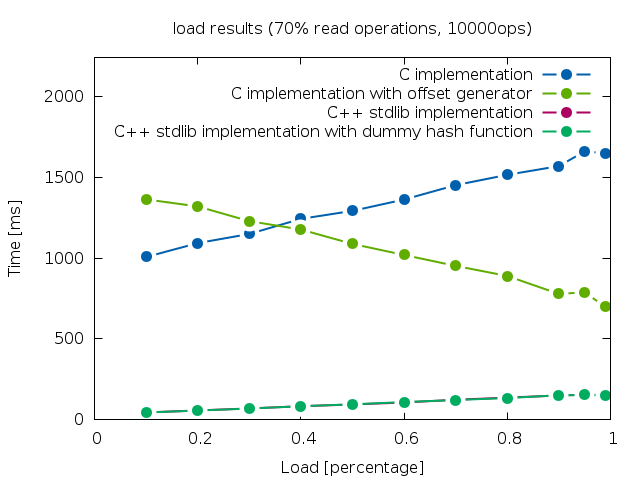
\includegraphics[width=0.9\textwidth]{result_example_contains.png}	
	\end{center}
\end{frame}

\begin{frame}
	\frametitle{Result -- only existing}
	\begin{center}
		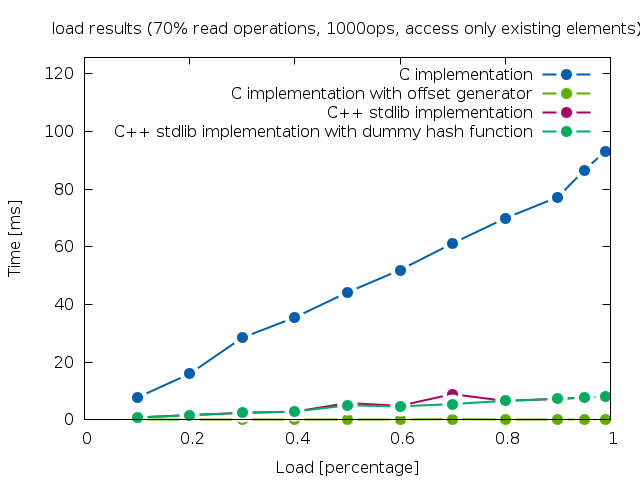
\includegraphics[width=0.9\textwidth]{result_example_no_contains.png}	
	\end{center}
\end{frame}


\section{Verification}
\subsection{What to prove ?}
\begin{frame}
	\frametitle{What to prove ?}
	\begin{center}
		Goal: show that increment by offset covers all the map.
	\end{center}
	\begin{itemize}
		\item Not always true (chinese remainder theorem).
		\item Requires: \texttt{offset} and \texttt{capacity} coprime ($gcd = 1$) (necessary and sufficient).
	\end{itemize}
\end{frame}

\begin{frame}
	\frametitle{What to prove ?}
	Insert \texttt{key4}: $h_1(\mathtt{key4}) = 5$, $h_2(\mathtt{key4}) = 2$: search empty ?
	\begin{center}
		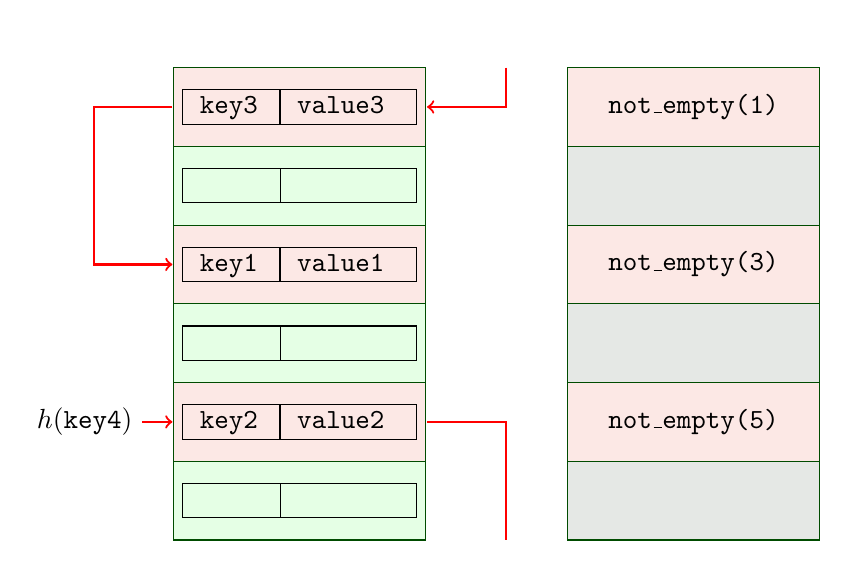
\begin{tikzpicture}
			\draw (0, -5) node[anchor=east] (key4) {$h(\mathtt{key4})$};

			\drawstruct{(7,0)}
			\structcell[occupiedcell]{\texttt{not\_empty(1)}} ;
			\structcell[padding]{} ;
			\structcell[occupiedcell]{\texttt{not\_empty(3)}} ;
			\structcell[padding]{} ;
			\structcell[occupiedcell]{\texttt{not\_empty(5)}} ;
			\structcell[padding]{} ;

			\drawstruct{(2,0)}
			\structcell[occupiedcell]{\keyvalue{key3}{value3}} \coordinate(firstCell) at (currentcell.west); \coordinate(firstCellOut) at (currentcell.east);
			\structcell[freecell]{\keyvalue{}{}} \coordinate(secondCell) at (currentcell.west); \coordinate (secondCellOut) at (currentcell.east);
			\structcell[occupiedcell]{\keyvalue{key1}{value1}} \coordinate(thirdCell) at (currentcell.west); \coordinate(thirdCellOut) at (currentcell.east);
			\structcell[freecell]{\keyvalue{}{}} \coordinate(fourthCell) at (currentcell.west); \coordinate (fourthCellOut) at (currentcell.east);
			\structcell[occupiedcell]{\keyvalue{key2}{value2}} \coordinate(fifthCell) at (currentcell.west); \coordinate(fifthCellOut) at (currentcell.east);
			\structcell[freecell]{\keyvalue{}{}} \coordinate(sixthCell) at (currentcell.west); \coordinate (sixthCellOut) at (currentcell.east);

			\draw[->, red, thick] (key4) -- (fifthCell);
			\draw[red, thick] (fifthCellOut) -| ++(1, -1.5) ;
			\draw[->, red, thick] (firstCellOut)+(1, 0.5) |-(firstCellOut);
			\draw[->, red, thick] (firstCell) -- ++(-1, 0) |- (thirdCell);

		\end{tikzpicture}
	\end{center}
\end{frame}

\subsection{Proof steps}
\begin{frame}
	\frametitle{Proof steps}
	If the number of iteration is less than the capacity: 
	\begin{itemize}
		\item Build and updated a \texttt{list<option<nat>>} with the same pattern.
		\item Each cell is: 
			\begin{itemize}
				\item \texttt{some(n)} if accessed after $n$ iterations.
				\item \texttt{none} if not accessed.
			\end{itemize}
		\item Apply Chinese Remainder Theorem.
		\item Deduce that only \texttt{none} are updated to \texttt{some}.
		\item Hence, the number of \texttt{some} is the number of iteration.
		\item For \texttt{capacity} iteration, all cells are \texttt{some}.
	\end{itemize}
\end{frame}

\begin{frame}
		If \texttt{some(n)}, then \texttt{prop(start+offset*n \% capa)}.
	\begin{center}
		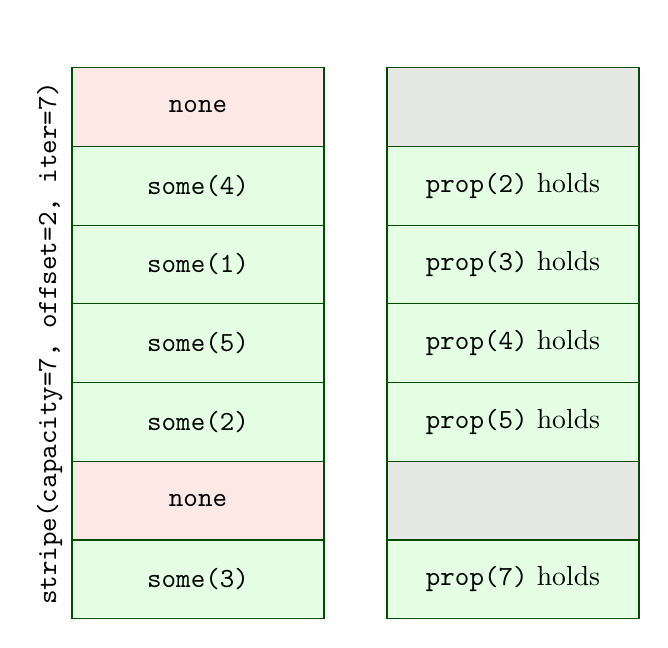
\begin{tikzpicture}
			\frametitle{Proof steps}
			\drawstruct{(0,0)}
			\structcell[occupiedcell]{\texttt{none}} ;
			\structcell[freecell]{\texttt{some(4)}} ;
			\structcell[freecell]{\texttt{some(1)}} ;
			\structcell[freecell]{\texttt{some(5)}} ;
			\structcell[freecell]{\texttt{some(2)}} ;
			\structcell[occupiedcell]{\texttt{none}} ;
			\structcell[freecell]{\texttt{some(3)}} ;
			\structname{\texttt{stripe(capacity=7, offset=2, iter=7)}};

			\drawstruct{(4,0)}
			\structcell[padding]{} ;
			\structcell[freecell]{\texttt{prop(2)} holds} ;
			\structcell[freecell]{\texttt{prop(3)} holds} ;
			\structcell[freecell]{\texttt{prop(4)} holds} ;
			\structcell[freecell]{\texttt{prop(5)} holds} ;
			\structcell[padding]{} ;
			\structcell[freecell]{\texttt{prop(7)} holds} ;
		\end{tikzpicture}
	\end{center}

\end{frame}
\begin{frame}
	\frametitle{Proof steps}


	\begin{columns}
		\begin{column}{0.5\textwidth}
			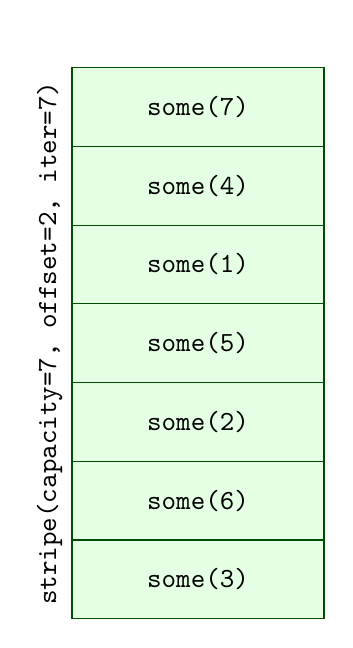
\begin{tikzpicture}
				\drawstruct{(0,0)}
				\structcell[freecell]{\texttt{some(7)}} ;
				\structcell[freecell]{\texttt{some(4)}} ;
				\structcell[freecell]{\texttt{some(1)}} ;
				\structcell[freecell]{\texttt{some(5)}} ;
				\structcell[freecell]{\texttt{some(2)}} ;
				\structcell[freecell]{\texttt{some(6)}} ;
				\structcell[freecell]{\texttt{some(3)}} ;
				\structname{\texttt{stripe(capacity=7, offset=2, iter=7)}};
			\end{tikzpicture}
		\end{column}
		\begin{column}{0.5\textwidth}
			$\Rightarrow \mathtt{count\_some = iter = 7}$\\
			$\Rightarrow$ All cells are \texttt{some}.
		\end{column}
	\end{columns}
\end{frame}

\begin{frame}
	\frametitle{Chinese Remainder Theorem}
	\begin{itemize}
		\item Requires to compute $gcd$ and prove its properties.
		\item Almost proved.
		\item Last assumption: Coprime factorization lemma ($a\bot c \wedge b\bot c \Rightarrow (a\cdot b)\bot c$).
	\end{itemize}
\end{frame}

\section{Conclusion}
\subsection{Hash Table software}
\begin{frame}
	\frametitle{Hash-Table software}
	\begin{itemize}
		\item Efficient (when key is present).
		\item Formally verified.
		\item Requires \texttt{capacity} and \texttt{offset} coprime.
	\end{itemize}
\end{frame}

\subsection{Remaining work}
\begin{frame}
	\frametitle{Remaining work}
	\begin{itemize}
		\item Coprime factorization lemma: $a\bot c \wedge b\bot c \Rightarrow (a\cdot b)\bot c$
		\item Logical operations (\texttt{shift} and \texttt{bitwise\_and})
		\item Some typing errors
	\end{itemize}
\end{frame}
\subsection{Side effects}
\begin{frame}
	\frametitle{Side effects}
	\begin{itemize}
		\item 6 commits in Verifast tree (\texttt{long long} support).
		\item 9 issues on Verifast.
		\item A random access sequence generator \& benchmark.
	\end{itemize}
\end{frame}



\begin{frame}
	\begin{center}
		\huge{Q\&A}
	\end{center}
\end{frame}

\end{document}
